\documentclass{article}
\usepackage{graphicx} % Required for inserting images
\usepackage{amsthm,amsmath,amssymb}
\usepackage[UTF8]{ctex}
\usepackage[tc]{titlepic}
\usepackage{titlesec}
\usepackage{cite}
\usepackage{fancyhdr}
\usepackage{booktabs}
\usepackage{subfigure}
\usepackage{float}
\usepackage[textwidth=14.5cm]{geometry}
\usepackage[section]{placeins}
\usepackage{makeidx}
\usepackage{mathrsfs}
\usepackage{color}
\usepackage{ulem}
\usepackage{enumitem}
\geometry{a4paper,scale=0.8,left=2cm,right=2cm}
\pagestyle{fancy}
\usepackage{microtype}
\usepackage{hyperref}
\usepackage{tcolorbox}
\usepackage{listings}

\lstset{
    language=Python, % 指定编程语言,如 Python、Java、C++ 等
    basicstyle=\footnotesize\ttfamily, % 调小字体大小
    keywordstyle=\color{blue}, % 关键字颜色
    commentstyle=\color{green!50!black}, % 注释颜色
    stringstyle=\color{red}, % 字符串颜色
    numbers=left, % 行号显示位置,left 表示在左侧显示
    numberstyle=\tiny\color{gray}, % 行号字体样式
    stepnumber=1, % 行号递增步长
    numbersep=5pt, % 行号与代码之间的间距
    backgroundcolor=\color{gray!10}, % 代码块背景颜色
    showspaces=false, % 不显示空格
    showstringspaces=false, % 不显示字符串中的空格
    showtabs=false, % 不显示制表符
    tabsize=2 % 制表符宽度
}


% 定义一个自定义命令,参数 #1 为中间的文字
\newcommand{\sectiondivider}[1]{%
  \vspace{1em} % 上下间距,可根据需要调整
  \begin{center}
    \noindent
    \makebox[0.3\linewidth]{\hrulefill}%
    \hspace{0.5em}% 左右间距
    {\Large\textbf{#1}}%
    \hspace{0.5em}%
    \makebox[0.3\linewidth]{\hrulefill}%
  \end{center}
  \vspace{3em}
}


\lhead{第 2 次作业\\\today}
\chead{中国科学技术大学\\	DS4001 人工智能原理与技术}

\rhead{Homework 2\\ {\CTEXoptions[today=old]\today}}
\newcommand{\upcite}[1]{\textsuperscript{\cite{#1}}}

\titleformat*{\section}{\bfseries\Large}
\titleformat*{\subsection}{\bfseries\large}

\title{\bfseries DS4001-25SP-HW2:搜索}
\author{刘芮希\quad PB22010402}

\begin{document}
%\begin{sloopypar}
\maketitle
% \clearpage


% Problem 1
\section{问题 1:马尔可夫决策过程[9\%=6\%+3\%]}

\begin{enumerate}[label=(\alph*), start=1]
    
    \item 迭代计算
    
    值迭代核心公式为$$V_{k+1}(s) = \max_{a} \left[ \sum_{s'} P(s' \mid s,a) \left( R(s,a,s') + \gamma V_k(s') \right) \right]$$
    下面进行数值计算
    
    \textbf{初始值:}$V^{(0)}(-2) = 0,
    V^{(0)}(-1) = 0,
    V^{(0)}(0) = 0,
    V^{(0)}(1) = 0,
    V^{(0)}(2) = 0$
    
    
    i=0 到 i=1:
    
    状态 -1:动作 $a_1$ 的 Q 值为 0.7×10 + 0.2×(-1) + 0.1×(-1) = 6.7,动作 $a_2$ 的 Q 值为 0.5×10 + 0.3×(-1) + 0.2×(-1) = 4.5,取最大值 6.7。
    
    状态 0:无论动作 $a_1$ 或 $a_2$,Q 值均为 -1.0(转移概率加权后均为负值),取 -1.0。
    
    状态 1:动作 $a_1$ 的 Q 值为 0.2×20 + 0.7×(-1) + 0.1×(-1) = 3.2,动作 $a_2$ 的 Q 值为 0.3×20 + 0.5×(-1) + 0.2×(-1) = 5.3,取最大值 5.3。
    
    \textbf{则}$V^{(1)}(-2) = 0,
    V^{(1)}(-1) = 6.7,
    V^{(1)}(0) = -1.0,
    V^{(1)}(1) = 5.3,
    V^{(1)}(2) = 0$
    
    i=1 到 i=2:
    
    状态 -1:动作 $a_1$ 的 Q 值为 $0.7×10 + 0.2×(-1 + V^{(1)}(0)) + 0.1×(-1 + V^{(1)}(-1)) = 7.17$,动作  $a_2$ 的 Q 值为 $0.5×10 + 0.3×(-1 + V^{(1)}(0)) + 0.2×(-1 + V^{(1)}(-1)) = 5.54$,取最大值 7.17。
    
    状态 0:动作 $a_1$ 的 Q 值为 $0.2×(-1 + V^{(1)}(1)) + 0.1×(-1 + V^{(1)}(0)) + 0.7×(-1 + V^{(1)}(-1)) = 4.65$,动作 $a_2$ 的 Q 值为 $0.3×(-1 + V^{(1)}(1)) + 0.2×(-1 + V^{(1)}(0)) + 0.5×(-1 + V₁(-1)) = 3.74$,取最大值 4.65。
    
    状态 1:动作 $a_1$ 的 Q 值为 $0.2×20 + 0.1×(-1 + V^{(1)}(1)) + 0.7×(-1 + V^{(1)}(0)) = 3.03$,动作 $a_2$ 的 Q 值为 $0.3×20 + 0.2×(-1 + V^{(1)}(1)) + 0.5×(-1 + V^{(1)}(0)) = 5.86$,取最大值 5.86。
    
    \textbf{则}$V^{(2)}(-2) = 0,
    V^{(2)}(-1) = 7.17,
    V^{(2)}(0) = 4.65,
    V^{(2)}(1) = 5.86,
    V^{(2)}(2) = 0$
    
    \item $i=2$ 时最优策略
    
    $s=-1$时,动作 $a_1$ 的 Q 值为7.17,动作  $a_2$ 的 Q 值为5.54,最优策略$\mu(-1)=a_1$
    
    $s=0$时,动作 $a_1$ 的 Q 值为4.65,动作  $a_2$ 的 Q 值为3.74,最优策略$\mu(0)=a_1$
    
    $s=1$时,动作 $a_1$ 的 Q 值为3.03,动作  $a_2$ 的 Q 值为5.86,最优策略$\mu(1)=a_2$
    
    $(s,\mu(s))$ 数值对为 $(-1,a_1),(0,a_1),(1,a_2)$
 
\end{enumerate}
\

% Problem 2
\section{问题 2:Q-Learning[12\%=3\%+6\%+3\%]}

\begin{enumerate}[label=(\alph*), start=1]

    \item 推导 $Q(s,a)$
    
    动作价值函数的定义为 $Q(s,a) = \mathbb{E} \left[ G_t \mid s_t = s, a_t = a \right]$ ,其中 $G_t = \sum_{k=t}^{\infty} \gamma^{k-t} R_k$
    
    执行动作 a 后,环境转移到状态 $s'$,获得即时奖励 $R(s,a,s')$,后续回报为 $\gamma G_{t+1}$ 。因此:
    $$\mathbb{E} \left[ G_t \mid s_t = s, a_t = a \right] = \mathbb{E} \left[ R(s,a,s') + \gamma G_{t+1} \mid s_t = s, a_t = a \right]$$
    
    对所有可能的下一状态 $s'$ ,计算其期望:
    $$\mathbb{E} \left[ R(s,a,s') + \gamma G_{t+1} \mid s_t = s, a_t = a \right] = \sum_{s'} P(s' \mid s,a) \left[ R(s,a,s') + \gamma \mathbb{E} \left[ G_{t+1} \mid s_{t+1} = s' \right] \right]$$
    
    根据状态价值函数的定义$ V(s') = \mathbb{E} \left[ G_{t+1} \mid s_{t+1} = s' \right]$代入得:
    $$\sum_{s'} P(s' \mid s,a) \left[ R(s,a,s') + \gamma \mathbb{E} \left[ G_{t+1} \mid s_{t+1} = s' \right] \right] = \sum_{s'} P(s' \mid s,a) \left( R(s,a,s') + \gamma V(s') \right)$$
    故 $Q(s,a) = \sum_{s'} P(s' \mid s,a) \left( R(s,a,s') + \gamma V(s') \right)$
    
    \item Monte-Carlo更新过程
    
    初始值 \( q(s, a) = 0 \),折扣因子 \( \gamma = 1 \),学习率 \( \alpha = 1 \)。轨迹为:
    \[
    \tau = \{(0, a_1, 2), (1, a_1, 3), (0, a_2, -1), (1, a_2, 0)\}
    \]
    
    \( t = 1 \)
    
    轨迹片段:\( (s=0, a=a_1, r=2) \)  
    
    计算回报 \( G_1 \):
    \[
    G_1 = 2 + 3 + (-1) + 0 = 4
    \]
    更新动作价值函数:
    \[
    q(0, a_1) \leftarrow G_1 = 4
    \]
    更新后的 \( q \)-表:
    \[
    \begin{array}{|c|c|c|}
    	\hline
    	s & a_1 & a_2 \\
    	\hline
    	0 & 4 & 0 \\
    	1 & 0 & 0 \\
    	\hline
    \end{array}
    \]
    
    \( t = 2 \)
    
    轨迹片段:\( (s=1, a=a_1, r=3) \)  
    
    计算回报 \( G_2 \):
    \[
    G_2 = 3 + (-1) + 0 = 2
    \]
    更新动作价值函数:
    \[
    q(1, a_1) \leftarrow G_2 = 2
    \]
    更新后的 \( q \)-表:
    \[
    \begin{array}{|c|c|c|}
    	\hline
    	s & a_1 & a_2 \\
    	\hline
    	0 & 4 & 0 \\
    	1 & 2 & 0 \\
    	\hline
    \end{array}
    \]
    
    \( t = 3 \)
    
    轨迹片段:\( (s=0, a=a_2, r=-1) \)  
    
    计算回报 \( G_3 \):
    \[
    G_3 = -1 + 0 = -1
    \]
    更新动作价值函数:
    \[
    q(0, a_2) \leftarrow G_3 = -1
    \]
    更新后的 \( q \)-表:
    \[
    \begin{array}{|c|c|c|}
    	\hline
    	s & a_1 & a_2 \\
    	\hline
    	0 & 4 & -1 \\
    	1 & 2 & 0 \\
    	\hline
    \end{array}
    \]
    
    \( t = 4 \)
    
    轨迹片段:\( (s=1, a=a_2, r=0) \)  
    
    计算回报 \( G_4 \):
    \[
    G_4 = 0
    \]
    更新动作价值函数:
    \[
    q(1, a_2) \leftarrow G_4 = 0
    \]
    最终 \( q \)-表:
    \[
    \begin{array}{|c|c|c|}
    	\hline
    	s & a_1 & a_2 \\
    	\hline
    	0 & 4 & -1 \\
    	1 & 2 & 0 \\
    	\hline
    \end{array}
    \]
    各时间步更新后的动作价值函数值:
    \[
    \begin{aligned}
    	& t=1: \quad q(0, a_1) = 4 \\
    	& t=2: \quad q(1, a_1) = 2 \\
    	& t=3: \quad q(0, a_2) = -1 \\
    	& t=4: \quad q(1, a_2) = 0 \\
    \end{aligned}
    \]
    
    \item Q-Learning 收敛性核心思路
    	
    Q-Learning 算法能够收敛的核心原因在于其通过 \textbf{贝尔曼最优算子的收缩性} 和 \textbf{状态-动作对的充分探索},逐步缩小估计值与最优值之间的误差,最终收敛到最优动作价值函数 \( Q^* \)。
    	
    1. 贝尔曼最优算子的收缩性
    
    Q-Learning 的更新本质是反复应用 \textbf{贝尔曼最优算子} \(\mathcal{T}\),其定义为:
    \[(\mathcal{T} Q)(s, a) = R(s, a) + \gamma \max_{a'} Q(s', a')\]
    该算子具有 \textbf{压缩映射} 性质,即对任意两个函数 \( Q_1 \) 和 \( Q_2 \),满足:
    \[\|\mathcal{T} Q_1 - \mathcal{T} Q_2\|_\infty \leq \gamma \|Q_1 - Q_2\|_\infty\]
    由于 \(\gamma \in [0, 1)\),每次应用算子后,函数之间的最大差异会以 \(\gamma\) 的倍数衰减。反复迭代后,Q 值会逐渐逼近唯一的不动点 \( Q^* \),即最优动作价值函数。
    	
    2. 误差的指数衰减
    
    假设初始 Q 表与 \( Q^* \) 的最大误差为 \(\Delta_0\),每次更新后,误差会被压缩为 \(\gamma \Delta_0\)。在 \textbf{确定性环境} 中,若每个状态-动作对 \((s, a)\) 被 \textbf{无限次访问},经过 \( k \) 轮遍历所有状态-动作对后,最大误差降至 \(\gamma^k \Delta_0\)。当 \( k \to \infty \),误差趋近于零,Q 表收敛到 \( Q^* \)。
    	
    3. 步长条件与推广
    	
    对于步长 \(\alpha \in (0, 1]\),更新公式可视为当前估计值与贝尔曼目标的加权平均:
    \[Q_{n+1}(s, a) = (1-\alpha) Q_n(s, a) + \alpha \mathcal{T} Q_n(s, a)\]
    在满足 \textbf{无限次访问条件} 时,误差上界变为 \((\alpha \gamma + 1 - \alpha)^k \Delta_0\)。由于 \(\alpha \gamma + (1 - \alpha) < 1\),误差仍以指数速率衰减,保证收敛。
    	
    4. 收敛前提条件
    \begin{itemize}
  		\item \textbf{有限 MDP}:状态与动作空间有限。
   		\item \textbf{充分探索}:每个状态-动作对被无限次访问(如通过 \(\epsilon\)-贪心策略)。
   		\item \textbf{确定性环境}:状态转移和奖励函数确定(可推广至非确定性环境,但需额外条件)。    
   	\end{itemize}
    	
    Q-Learning 的收敛性依赖于 \textbf{贝尔曼算子的压缩性} 和 \textbf{状态-动作对的充分探索},通过迭代逐步消除估计误差,最终逼近最优策略。其本质是通过动态规划的收缩过程,结合增量式更新,实现对长期回报的准确估计。
    
    
\end{enumerate}
\

% Problem 3
\section{问题 3:Gobang Programming[53\%=33\%+10\%+10\%]}


\begin{enumerate}[label=(\alph*), start=1]
    \item \textbf{[代码]} %3a
    % get_next_state 5分
    \begin{lstlisting}[language=Python]
def get_next_state(self, action: Tuple[int, int, int], noise: Tuple[int, int, int]) -> np.array:
		next_state = self.board.copy() 
		piece, x, y = action
		next_state[x][y] = piece

		if noise is not None:
				white, x_white, y_white = noise
				next_state[x_white][y_white] = white
		return next_state
    \end{lstlisting}
    
    % sample_noise 3分
    \begin{lstlisting}[language=Python]
def sample_noise(self) -> Union[Tuple[int, int, int], None]:
		if self.action_space:
				x, y = random.choice(self.action_space)
				self.action_space.remove((x, y))
				return 2, x, y
		else:
				return None
    \end{lstlisting}

    % get_connection_and_reward 5分
    \begin{lstlisting}[language=Python]
def get_connection_and_reward(self, action: Tuple[int, int, int], 
noise: Tuple[int, int, int]) -> Tuple[int, int, int, int, float]:
		black_1, white_1 = self.count_max_connections(self.board)
		next_state = self.get_next_state(action, noise)
		black_2, white_2 = self.count_max_connections(next_state)
		reward = (black_2 - black_1) - (white_2 - white_1)
		return black_1, white_1, black_2, white_2, reward
    \end{lstlisting}

    % sample_action_and_noise 8分
    \begin{lstlisting}[language=Python]
def sample_action_and_noise(self, eps: float):
    s = self.array_to_hashable(self.board)
    if random.random() < eps or s not in self.Q:
    		x, y = random.choice(self.action_space)
    		action = (1, x, y)
    else:
    		valid_actions = [(a, q) for a, q in self.Q[s].items() if (a[1], a[2]) in self.action_space]
    		if valid_actions:
    				action = max(valid_actions, key=lambda item: item[1])[0]
    		else:
    				x, y = random.choice(self.action_space)
    				action = (1, x, y)
    self.action_space.remove((action[1], action[2]))
    return action, self.sample_noise()
    \end{lstlisting}

    % q_learning_update 12分
    \begin{lstlisting}[language=Python]
def q_learning_update(self, s0_: np.array, action: Tuple[int, int, int], 
	s1_: np.array, reward: float,alpha_0: float = 1):
    s0, s1 = self.array_to_hashable(s0_), self.array_to_hashable(s1_)
    self.s_a_visited[(s0, action)] = 1 if (s0, action) not in self.s_a_visited else \
        self.s_a_visited[(s0, action)] + 1
    alpha = alpha_0 / self.s_a_visited[(s0, action)]
    if s0 not in self.Q:
    		self.Q[s0] = {}
    current_q = self.Q[s0].get(action, 0.0)
    if s1 in self.Q and self.Q[s1]:
    		max_q_next = max(self.Q[s1].values())
    else:
    		max_q_next = 0.0
    new_q = current_q + alpha * (reward + max_q_next - current_q)
    self.Q[s0][action] = new_q
    \end{lstlisting}

    \item n=3 训练及测试结果
    \FloatBarrier
    \begin{figure}[htbp]
    	\centering
    	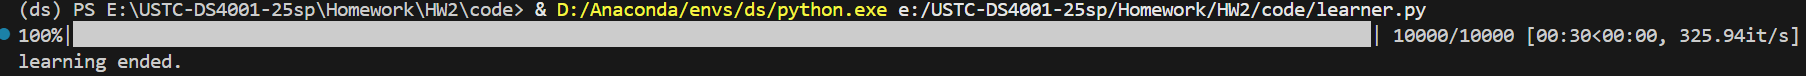
\includegraphics[width=\textwidth]{train3.png}
    	\caption{n=3训练}
    \end{figure}
    \begin{figure}[htbp]
    	\centering
    	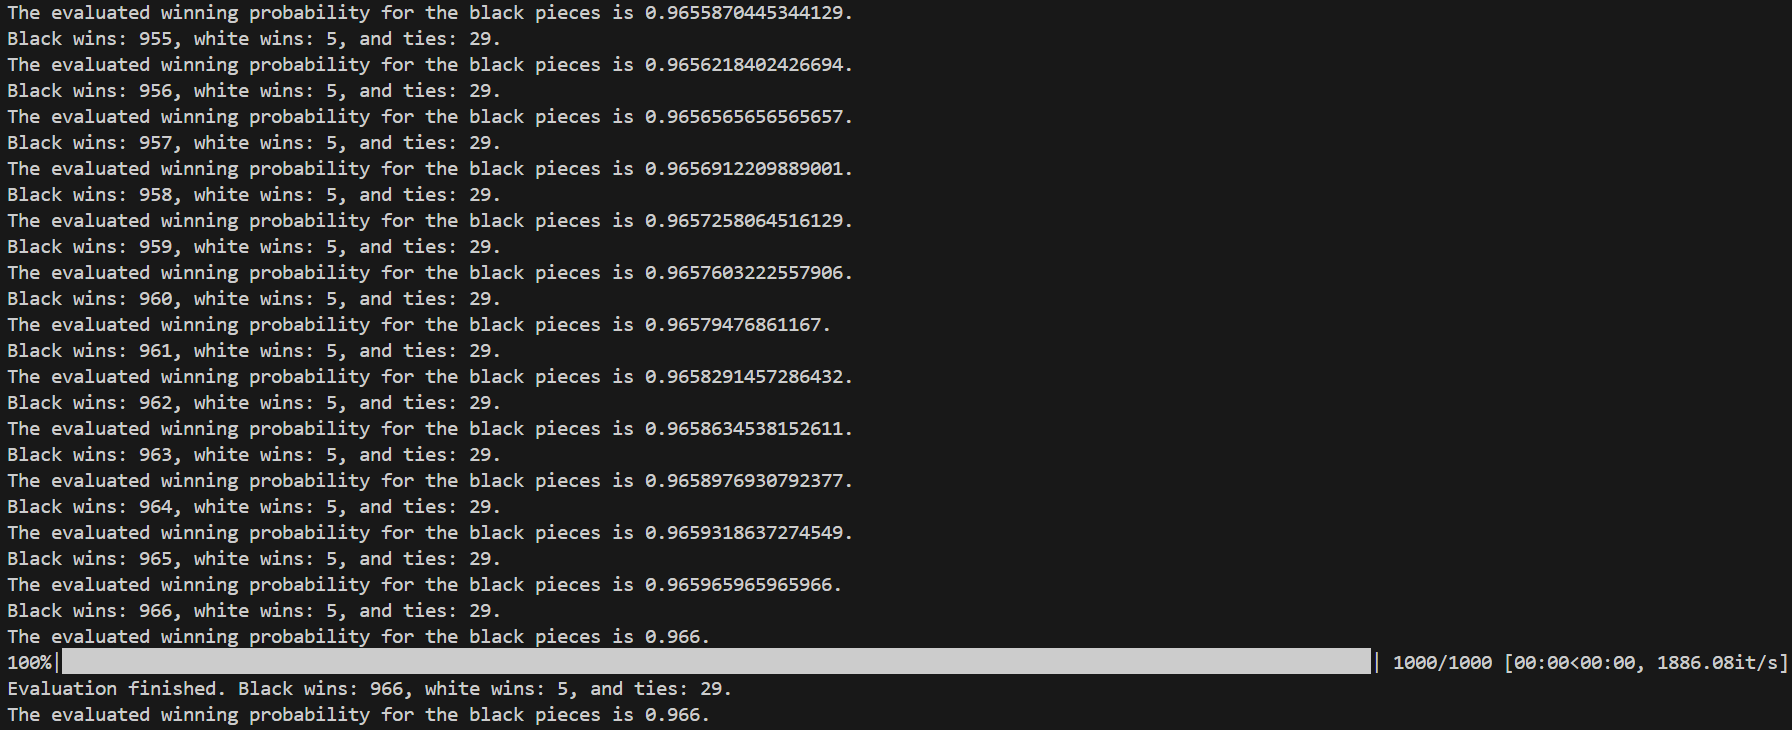
\includegraphics[width=0.8\textwidth]{test3.png}
    	\caption{n=3测试}
    \end{figure}
\FloatBarrier
    \item n=4 训练及测试结果
    \FloatBarrier
    \begin{figure}[htbp]
    	\centering
    	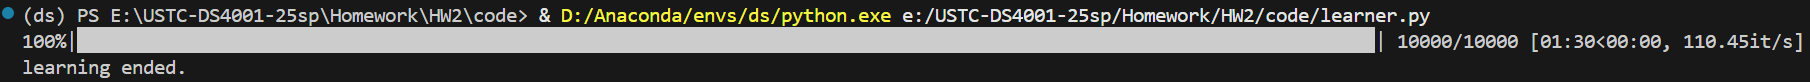
\includegraphics[width=\textwidth]{train4.png}
    	\caption{n=4训练}
    \end{figure}
    \begin{figure}[htbp]
    	\centering
    	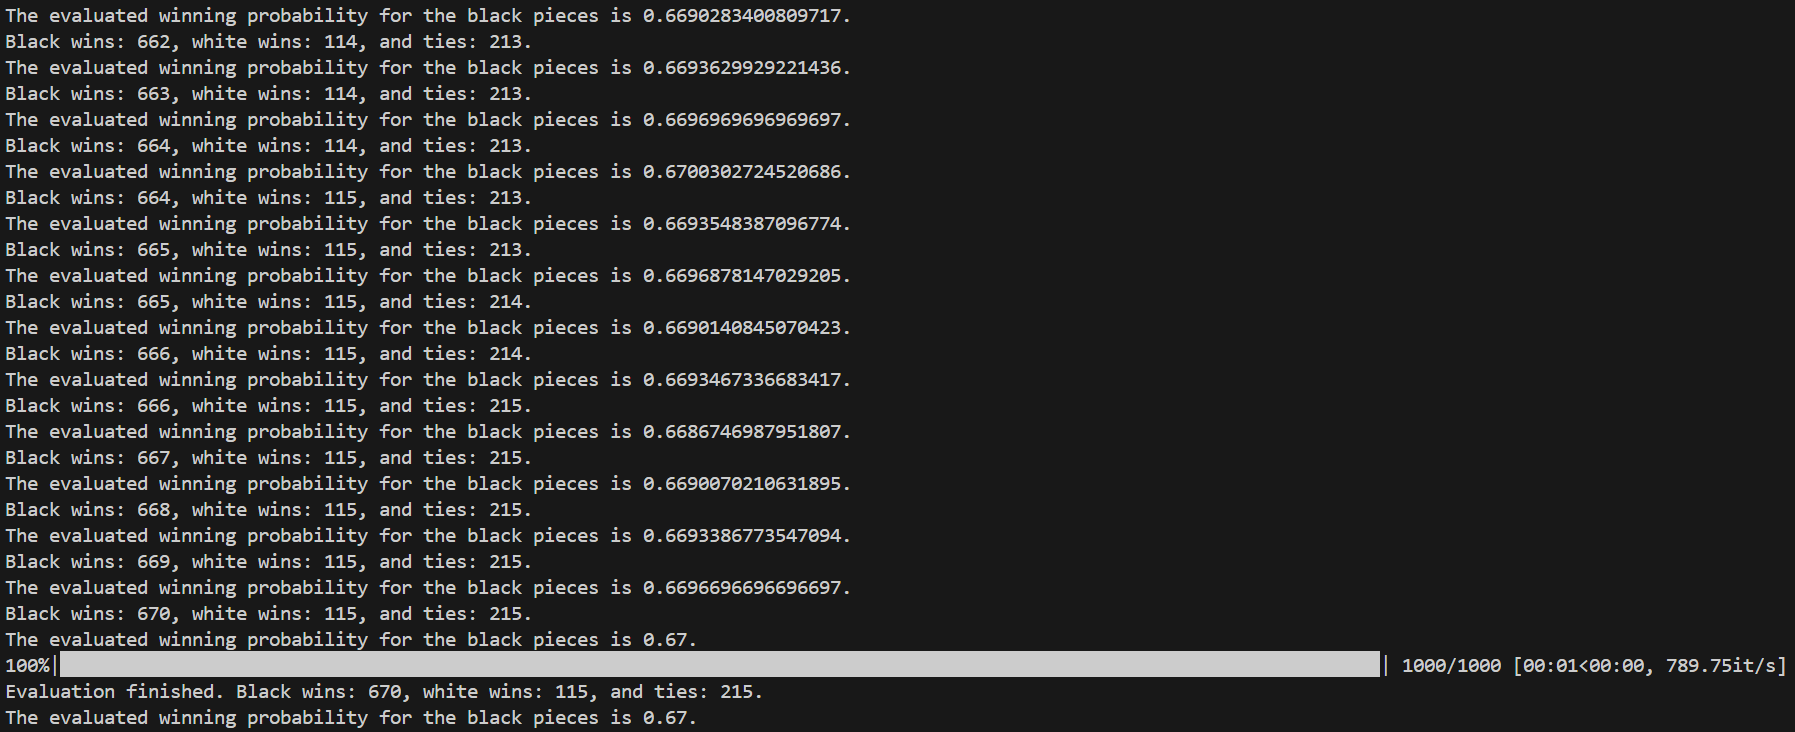
\includegraphics[width=0.8\textwidth]{test4.png}
    	\caption{n=4测试}
    \end{figure}
    \FloatBarrier
\end{enumerate}
\

% Problem 4
\section{问题 4:Deeper Understanding[16\%=5\%+5\%+2\%+4\%]}
\subsection{Bellman 算子与压缩映射}
\begin{enumerate}[label=(\alph*), start=1]
    
    \item 证明 Bellman 算子是压缩映射
    
    1. \textbf{定义 Bellman 算子}:
    \[
    (\mathcal{T}v)(s) = \max_{a \in A} \left\{ r_{sa} + \gamma \cdot \sum_{s' \in S} p_{sas'} \cdot v(s') \right\}.
    \]
    对于两个价值函数 \(v_1\) 和 \(v_2\),分别有:
    \[
    (\mathcal{T}v_1)(s) = \max_{a \in A} \left\{ r_{sa} + \gamma \cdot \sum_{s' \in S} p_{sas'} \cdot v_1(s') \right\},
    \]
    \[
    (\mathcal{T}v_2)(s) = \max_{a \in A} \left\{ r_{sa} + \gamma \cdot \sum_{s' \in S} p_{sas'} \cdot v_2(s') \right\}.
    \]
    
    2. \textbf{构造差值}:
    对于任意状态 \(s\),设 \(a_1^*\) 和 \(a_2^*\) 分别是使得 \(\mathcal{T}v_1\) 和 \(\mathcal{T}v_2\) 达到最大值的动作:
    \[
    (\mathcal{T}v_1)(s) = r_{sa_1^*} + \gamma \cdot \sum_{s' \in S} p_{sa_1^*s'} \cdot v_1(s'),
    \]
    \[
    (\mathcal{T}v_2)(s) = r_{sa_2^*} + \gamma \cdot \sum_{s' \in S} p_{sa_2^*s'} \cdot v_2(s').
    \]
    由于 \(a_1^*\) 是 \(v_1\) 下的最优动作,而 \(a_2^*\) 是 \(v_2\) 下的最优动作,因此:
    \[
    (\mathcal{T}v_1)(s) \geq r_{sa_2^*} + \gamma \cdot \sum_{s' \in S} p_{sa_2^*s'} \cdot v_1(s'),
    \]
    \[
    (\mathcal{T}v_2)(s) \geq r_{sa_1^*} + \gamma \cdot \sum_{s' \in S} p_{sa_1^*s'} \cdot v_2(s').
    \]
    利用这些不等式,可以得到:
    \[
    (\mathcal{T}v_1)(s) - (\mathcal{T}v_2)(s) \leq \gamma \cdot \sum_{s' \in S} p_{sa_2^*s'} (v_1(s') - v_2(s')) \leq \gamma \|v_1 - v_2\|_\infty,
    \]
    \[
    (\mathcal{T}v_2)(s) - (\mathcal{T}v_1)(s) \leq \gamma \cdot \sum_{s' \in S} p_{sa_1^*s'} (v_2(s') - v_1(s')) \leq \gamma \|v_1 - v_2\|_\infty.
    \]
    因此:
    \[
    |(\mathcal{T}v_1)(s) - (\mathcal{T}v_2)(s)| \leq \gamma \|v_1 - v_2\|_\infty.
    \]
    
    3. \textbf{取最大值}:
    对所有状态 \(s\) 取最大值,得到:
    \[
    \|\mathcal{T}v_1 - \mathcal{T}v_2\|_\infty = \max_{s \in S} |(\mathcal{T}v_1)(s) - (\mathcal{T}v_2)(s)| \leq \gamma \|v_1 - v_2\|_\infty.
    \]
    
    综上,Bellman 算子 \(\mathcal{T}\) 是最大范数下的 \(\gamma\)-压缩映射。
    
    \item 证明最多一个不动点
    
    假设存在两个不同的不动点 $v_1$ 和 $v_2$,即:
    \[
    \mathcal{T}v_1 = v_1, \quad \mathcal{T}v_2 = v_2.
    \]
    
    根据 $\gamma$-压缩性质,有:
    \[
    \|v_1 - v_2\|_\infty = \|\mathcal{T}v_1 - \mathcal{T}v_2\|_\infty \leq \gamma \|v_1 - v_2\|_\infty.
    \]
    
    整理得:
    \[
    (1 - \gamma)\|v_1 - v_2\|_\infty \leq 0.
    \]
    
    由于 $\gamma \in [0,1)$,故 $1 - \gamma > 0$,这意味着:
    \[
    \|v_1 - v_2\|_\infty \leq 0.
    \]
    
    而范数具有非负性,因此:
    \[
    \|v_1 - v_2\|_\infty = 0 \quad \Rightarrow \quad v_1 = v_2.
    \]
    
    这与假设 $v_1$ 和 $v_2$ 不同矛盾,故 $\mathcal{T}$ 最多只能有一个不动点。
\end{enumerate}

\subsection{重要性采样}
\begin{enumerate}[label=(\alph*), start=1]
    
    \item 重要性采样等式证明
    
    假设分布 \(q(x)\) 的支撑集包含 \(p(x)\) 的支撑集,即当 \(p(x) > 0\) 时,\(q(x) > 0\)。  
    若此条件不满足,则 \(\frac{p(x)}{q(x)}\) 在 \(q(x) = 0\) 时无定义,需额外处理。
    
    对于 \(x \sim p\) 的期望:  
    \begin{align}
    	\mathbb{E}_{x \sim p}[f(x)] 
    	&= \int f(x) \, p(x) \, \mathrm{d}x \quad \text{(连续情况)} \\
    	\text{或} \quad \mathbb{E}_{x \sim p}[f(x)] 
    	&= \sum_{x} f(x) \, p(x) \quad \text{(离散情况)}.
    \end{align}
    
    对右侧的 \(x \sim q\) 的期望进行展开:  
    \begin{align}
    	\mathbb{E}_{x \sim q}\left[f(x) \frac{p(x)}{q(x)}\right] 
    	&= \int f(x) \frac{p(x)}{q(x)} \, q(x) \, \mathrm{d}x \quad \text{(连续情况)} \\
    	\text{或} \quad \mathbb{E}_{x \sim q}\left[f(x) \frac{p(x)}{q(x)}\right] 
    	&= \sum_{x} f(x) \frac{p(x)}{q(x)} \, q(x) \quad \text{(离散情况)}.
    \end{align}
    
    在两种情况下,\(q(x)\) 与分母的 \(q(x)\) 抵消:  
    \begin{align}
    	\int f(x) p(x) \, \mathrm{d}x 
    	&= \mathbb{E}_{x \sim p}[f(x)] \quad \text{(连续情况)}, \\
    	\sum_{x} f(x) p(x) 
    	&= \mathbb{E}_{x \sim p}[f(x)] \quad \text{(离散情况)}.
    \end{align}
    
    在支撑集条件满足时,有:  
    \[
    \mathbb{E}_{x \sim p}[f(x)] = \mathbb{E}_{x \sim q}\left[f(x) \frac{p(x)}{q(x)}\right].
    \]
    
    \item 方差公式证明
    
    根据方差公式 \(\text{Var}[X] = \mathbb{E}[X^2] - (\mathbb{E}[X])^2\):
    \[
    \text{Var}_{x \sim p}[f(x)] = \mathbb{E}_{x \sim p}\left[f(x)^2\right] - \left(\mathbb{E}_{x \sim p}[f(x)]\right)^2,
    \]
    \[
    \text{Var}_{x \sim q}\left[f(x)\frac{p(x)}{q(x)}\right] = \mathbb{E}_{x \sim q}\left[\left(f(x)\frac{p(x)}{q(x)}\right)^2\right] - \left(\mathbb{E}_{x \sim q}\left[f(x)\frac{p(x)}{q(x)}\right]\right)^2.
    \]
    
    由重要性采样性质 \(\mathbb{E}_{x \sim q}\left[f(x)\frac{p(x)}{q(x)}\right] = \mathbb{E}_{x \sim p}[f(x)]\),可得:
    \[
    \left(\mathbb{E}_{x \sim q}\left[f(x)\frac{p(x)}{q(x)}\right]\right)^2 = \left(\mathbb{E}_{x \sim p}[f(x)]\right)^2.
    \]
    
    代入方差差表达式
    \[
    \begin{aligned}
    \text{Var}_{p}[f(x)] - \text{Var}_{q}\left[f(x)\frac{p(x)}{q(x)}\right] &= \left[\mathbb{E}_{p}[f(x)^2] - \left(\mathbb{E}_{p}[f(x)]\right)^2\right] \\
    &\quad - \left[\mathbb{E}_{q}\left[f(x)^2\frac{p(x)^2}{q(x)^2}\right] - \left(\mathbb{E}_{p}[f(x)]\right)^2\right] \\
    &= \mathbb{E}_{p}[f(x)^2] - \mathbb{E}_{q}\left[f(x)^2\frac{p(x)^2}{q(x)^2}\right].
    \end{aligned}
    \]
    
    利用重要性采样:
    \[
    \mathbb{E}_{q}\left[f(x)^2\frac{p(x)^2}{q(x)^2}\right] = \mathbb{E}_{p}\left[f(x)^2\frac{p(x)}{q(x)}\right].
    \]
    
    故\[
    \text{Var}_{p}[f(x)] - \text{Var}_{q}\left[f(x)\frac{p(x)}{q(x)}\right] = \mathbb{E}_{p}[f(x)^2] - \mathbb{E}_{p}\left[f(x)^2\frac{p(x)}{q(x)}\right].
    \]
    
\end{enumerate}
\

\section*{体验反馈[10\%]}

\begin{enumerate}[label=(\alph*), start=1]
    \item \textbf{[必做]} %所花时间
    8h
    \item \textbf{[选做]} %其他反馈
    我五子棋能下得过AI吗
\end{enumerate}


\end{document}
